\secnumbersection{SOLUTION PROPOSAL} \label{sec:prop}

The approach used to improve on the software's computing time followed a logical order.
First, the algorithm is exhaustively analyzed and profiled to find the bottlenecks in the execution, so as to be able to focus the work on them.
Then, the cause for each significant bottleneck is identified and investigated, so as to propose solutions using the state of the art in the field, and after a good understanding of each problem is reached, they are addressed.
Finally, thorough validation sessions are attempted so as to be sure that the changes made don't affect negative the software's results and to secure that the computing time is effectively reduced.

\subsection{Refactoring and Optimizations} \label{ssec:refactoring_and_optimizations} % \subsubsection{Code Clean-up} \label{sssec:cleanup}
Before any large change or algorithm implementation is considered on the software, it was decided to do a so-called ``code-cleanup''.
This was considered necessary mainly because of two reasons:

First, the current implementation had a low readability, presenting various issues like uneven indentation style, non-compliance with the Java code conventions~\cite{sun1997java}, inconsistent and arbitrary variable and method names, among many others.
This can be seen in the link to the original repository provided at Section \ref{add:code_and_reproducibility}.

The second reason is the large presence of many unintentional, unmanaged architectural technical debt (technical debts and their classification are explained briefly in Appendix \ref{add:technical_debt}).
% While most technical debts are invisible without a detailed analysis, the symptoms for many of them can be clear to most experienced programmers.
Many instances of these debts were found in the DC code, in the form of repeated portions of code, a general lack of error checking and reporting and a general lack of comments in difficult-to-understand sections of code, among others.

Due to both these reasons and simply to improve the author's familiarity with the code, the previously mentioned clean-up was done.
The measures implemented in this process are the following:

    \begin{itemize}
        \item \textbf{Addition of comments}: A comprehensive list of the segments of code with a non-intuitive purpose was written.
        A small research was then performed for each point in the list, looking into the math, physics or general algorithms from which it could be derived.
        When this was found, a comment was written either providing a small explanation or referring to the name of the formula or algorithm used.
        When this research was unfruitful, the original author of the code was contacted so that she could provide enough information about the code segment so as to write this explanatory comment (Contact information is given in Appendix \ref{add:code_and_reproducibility}).
    
        Apart from the general comments, a complete JavaDoc documentation was added to the most important classes and methods in the DC code, with sparse documentation added also to hard-to-understand classes or methods in less critical classes.
    
        \item \textbf{Indentation Consistency}: Considering that the indentation style at the DC software was very inconsistent, this was fixed to improve readability.
        Now, the ``ideal length'' of indentations and the use of tab characters or space characters for it has been a long-running debate between programmers, so instead of finding the ``best option'' for it, the current standard used in most of the CLAS12 codebase was implemented, which simply is four space characters per indent.
    
        \item \textbf{Line Length Fixes}: While the code doesn't follow a rigorous standard, a line length of $100$ characters can be seen somewhat consistently thorough the CLAS12 codebase, sticking to the java conventions~\cite{sun1997java}.
        This line length is not strictly applied to the DC code, but instead some extremely long ($>300$ characters) segments of code are separated into various lines to aid readability.
    
        \item \textbf{Class, Method and Variables Names}: The standard Java conventions stipulate a consistent camel case naming standard, and while most of the code follows this style, the DC code tends to stray away from it in many ways.
        These include variables in lower case with or without underscores, variables and methods starting with an underscore, methods starting with uppercase, etc.
        The standard naming convention is applied to all of these instances.
    \end{itemize}

\subsubsection{Refactoring}\label{sssec:refactoring}
By definition, refactoring is the art of safely improving the design of existing code without changing its behaviour.
Changes done to the code through refactoring do not add new functionalities or represent design improvements, but only work to eliminate or reduce \textbf{code \textit{smells}}. % Note: I feel like refactoring does add design improvements but the usual java documentation on this says that by definition they don't so idk.
Code \textit{smells} are warning signs about potential problems in the code, meaning points that are worthy of a revision~\cite{wake2004refactoring}.

A small list of some the code \textit{smells} found in the DC code together with examples and the treatment done follows.
It is worth noting that this list is far from comprehensive, and just lists the \textit{smells} relevant to the discussion:
    \begin{itemize}
        \item \textbf{Long Methods}: Many methods with a very large amount of lines can be found thorough the code.
        In a normal situation this wouldn't be considered to be a big issue, but in the case of DC, many of these large methods contain repeated code or very similar segments, which in itself is considered a problem since it breeds inconsistencies and longer implementation times to any change done to the code.
        
        An example of this is the method \texttt{RK4transport} from the class \texttt{RungeKutta}, from the package \texttt{org.jlab.rec.dc.track.fit}, which is $269$ lines long.
        It's worth mentioning that the algorithm implemented in this method is \textbf{Runge Kutta 4}, and is described in Section \ref{ssec:framework_rk4}.

        The treatment for this problem is easy to implement, and involves simply splitting the method.
        What is done to do this is to extract the repeating segments into their own private methods, allowing then the original method to call these new methods.
        The benefit of this change is the elimination of duplicated code and a large performance improvement due to the elimination of unnecessary loops, which is explained further in Section \ref{sssec:optimizations}.
    
        In the mentioned example, the method can be split into various methods: First, the computation of $k_1$, $k_2$, $k_3$ and $k_4$ can all be done in the same method, reducing $172$ lines of code into $4$ method calls, with the new method being only $45$ lines long.
        After this, the final $RK4$ computation can be left as is, and some extra steps done to compute the covariance matrix can all be split into their own methods, easing the future debugging of the method and allowing each computation to be changed or optimized separately.
        The final \texttt{RK4transport} method is left with a total of $33$ lines of code with $7$ method calls.
        It's worth noting that this number can be further reduced to $20$ lines by packing intermediary variables into arrays, but to avoid the danger of reducing code readability it was considered a good idea to avoid this option.

        \item \textbf{Long Parameter Lists}: Similar to the last \textit{smell}, long parameter lists can be found thorough the DC code.
        In most cases specific to the software in study, these lists are expressed in the form of a long list of inputs for methods.
        An example for this is the \texttt{getTrackInitFit} method in the class \texttt{TrackCandListFinder} contained in the \texttt{org.jlab.rec.dc.track} package, where $20$ parameters are given to the method.
        These parameters are the integer \texttt{sector}, a long list of doubles: \texttt{x1}, \texttt{y1}, \texttt{z1}, \texttt{x2}, \texttt{y2}, \texttt{z2}, \texttt{x3}, \texttt{y3}, \texttt{z3}, \texttt{ux}, \texttt{uy}, \texttt{uz}, \texttt{thX}, \texttt{thY}, \texttt{theta1}, \texttt{theta3}, \texttt{iBdl}, \texttt{TORSCALE}, and an instance of the \texttt{Swim} class.
    
        Fixing such issues is usually easy, just requiring some degree of packaging for the parameters.
        For the example given, the previosly mentioned method is called by \texttt{GetTrackCands}, another method from the same class.
        In this method, three \textbf{cross} objects are unpacked to obtain the first $14$ doubles from the mentioned list, with two more doubles coming from clusters contained in the crosses and finally \texttt{iBdl} coming from the trajectory formed by the crosses.
        These \textbf{cross} objects are sets of two clusters from adjacent superlayers, while the \texttt{iBdl} variables denotes the integral of the magnetic field. % Note: I don't know exactly what iBdl is but no sources I found say more than "Integral of the magnetic field" so at least apparently physicists get it.
        The \texttt{sector} integer mentioned can also be obtained from the first cross.
        As can be seen, the $20$ input parameters given to the method can be replaced with three \texttt{cross} objects, the \texttt{TORSCALE} value and the instance of the \texttt{Swim} class previously mentioned, reducing the parameter list to four objects and only one parameter. % Note: Maybe an UML diagram or something like it might be useful here.
    
        \item \textbf{Commented and Dead Code}: This \textit{smell} consists in the presence of commented code, and is usually caused by either old code that the programmer decided to leave commented instead of deleting in case that it becomes useful in the future.
        Dead code is the phenomena that occurs when new methods are written and old and unused methods are never deleted.
        Both commented and dead code segments are present in large quantities in the DC software, and after a meeting between the author and the programmer it was decided to simply remove all this code since analyzing which segments would be useful or not would probably be too large a task for the minimal benefit provided by doing it.

        \item \textbf{Duplicated Code}: This \textit{smell} is characterized by two or more code fragments that look almost or completely identical.
        Duplication usually occurs when multiple programmers are working on different parts of the same program at the same time, but in the case of the DC software this can be attributed to accidents. % Note: More elaboration here might be useful.
        The solution to this problem is fairly simple: extract the duplicated code, create a new method to run this code and have both instances call this new method.
    
        In the case of the DC software, there is one instance where code duplication is very easily spotted; both the \texttt{RoadFinder} class from the \texttt{org.jlab.rec.dc.trajectory} package and the \texttt{CrossListFinder.TrajectoryParametriz} class from the \texttt{org.jlab.rec.dc.cross} package contain the exact same method, even using the same name, \texttt{evaluate}, and the code in this method does the same: fit a set of points into a line and return the parameters of the fit along with the $\chi^2$ probability and the number of degrees of freedom. % Note: Maybe this paragraph is too angry.
    
        \item \textbf{Data Class}: The final \textit{smell} that will be discussed in this work is the so-called ``data class'' \textit{smell}, which refers to a class that contains only fields and setters and getters to access them.
        In the case of the DC codebase, an example of this would be both the \texttt{StateVec} and the \texttt{CovMat} classes from the \texttt{org.jlab.rec.dc.track.fit} package.
        Both classes just define a state vector (described in Section \ref{ssec:framework_tf}) and a covariance matrix (described in Appendix \ref{add:covariance_matrix}), without providing any methods apart from the basic definition of the concepts.
    
        The treatment for this problem is through the encapsulation of the data class inside another class, ideally one that uses it.
        In the example, both these classes were encapsulated in another class named \texttt{StateVecs} from the same package.
    \end{itemize}

\subsubsection{Optimizations}\label{sssec:optimizations}
While cleaning up and refactoring the code, many optimizations were applied to the critical areas described in Section \ref{ssec:prof_results} so as to accelerate the bottlenecks and speed up the whole CLAS12 software.
These optimizations involve the addition of variables to precompute results instead of calculating them several times, the reduction of complexity orders by removing unnecessary loops, and the improvements brought by simply restructuring the code as described in the last Section.

% Note: Here I could talk about how the precomputation of results helped (and they helped a ton), and how to do the reduction of complexity with examples, especially considering the massive changes in performance this step brought to the code. I'd need some references for this, but I'm afraid I can't find much on that. % TODO: Implement the examples given here in the code.
\newpage
\subsection{Matrices Handling Changes} \label{ssec:prop_matrices}
% NOTE: Maybe this could use a plot?
Based on the profiling analysis shown in Section \ref{ssec:val_refactoring_and_optimizations}, This section focuses on reducing the CPU time of both the \texttt{isNonSingular} and the \texttt{filter} methods, which are explained in the \textbf{Update} segment of Section \ref{ssec:framework_ekf}.
For the calculation of the computational cost of mathematical operations, it is assumed that all ``basic'' operations: summation, subtraction, multiplication and division have a cost of $O(1)$.
The reasoning behind this decision is described in Appendix \ref{add:flops}.

It's worth noting that a very usual approach for accelerating matrix operations at the time of writing is leveraging the computation to GPUs, and it has been commonly used in particular to accelerate the KF itself~\cite{huang2011accelerating,blattner2011performance}.
This approach is not considered useful for CLAS12 because the matrices that are being handled are very small (the covariance matrix is only $5\times5$) and it is easy to realize that the time used to leverage the matrices to a GPU would likely make the software slower than the current implementation due to the time consumed in the memory transfer overhead~\cite{moravanszky2003dense}.

In the same spirit, neither the Strassen~\cite{strassen1969gaussian} or the Coppersmith-Winograd~\cite{coppersmith1990matrix} algorithms are considered to replace matrix multiplications or inversions since they're only useful for large matrices~\cite{ballard2012communication}.
As an example, the actual amount of operations required for computing the Strassen algorithm is $n^2 + n^{2.807}$, which for the case of a $5\times5$ matrix is $\sim117$ contrasted with the $125$ required by the na\"ive implementation and adding additional numerical instability~\cite{ballard2012communication}.
This reduction is small when compared with the specific optimizations that are described below, which eliminate matrix multiplication altogether for the methods brought into attention.

\subsubsection{Matrix Inverse} \label{sssec:prop_matrix_inverse}

To reduce the time spent by the update phase or filter method, the effort was mainly focused in the reduction of the time it takes to calculate the covariance matrix \textit{a posteriori} as seen in Equation \eqref{eq:ekf_Pk}.
The specific implementation of the equation presented in that section for the DC software is the following:

First, the determinant of the covariance matrix $P_{k|k-1}$ is computed and compared with $0$ to drop the track if the matrix is singular or near-singular.
Then, using the measurement data described in Section \ref{ssec:framework_tf}, the vector $\mathbf{h}_k$ is defined as:
    \begin{equation}
        \mathbf{h}_k = \begin{pmatrix}1\\ -\text{tan}(6t) - \frac{4w}{l}(1 - \frac{2y}{l})\\ 0\\ 0\\ 0\end{pmatrix}\,, \label{eq:mhc_hvec}
    \end{equation}
which is simply defined to project the state vector and covariance matrix to the tilted coordinate system from which the measurement is obtained.
From this, the matrix $P_{k|k}$ is computed as:
    \begin{equation}
        P_{k|k} = (P_{k|k-1}^{-1} + H_k)^{-1}\,, \label{eq:mhc_Pk}
    \end{equation}
where $H_k = \mathbf{h}_k^T\mathbf{h}_k$.
Finally, the $P_{k|k}$'s determinant is compared with $0$, again to drop the track if the new covariance matrix is singular.

To reduce the computation time of this calculation, the \textbf{Sherman-Morrison formula} (described in Appendix \ref{add:shermanmorrison_formula}) can be applied as long as $|P_{k|k-1}|\neq 0$~\cite{sherman1950adjustment}.
Applying the formula to Equation \eqref{eq:mhc_Pk}:
    \begin{equation}
        P_{k|k} = P_{k|k-1} - \frac{P_{k|k-1} \mathbf{h}_k \mathbf{h}_k^T P_{k|k-1}}{1 + \mathbf{h}_k^T P_{k|k-1} \mathbf{h}_k}\,. \label{eq:mhc_sm_det}
    \end{equation}
This helps to heavily reduce the total computation time since, as can be seen in the equation, no matrix inversions are required, which are very heavy operations~\cite{fatahalian2004understanding}.
It's worth noting that for this approach to be effective, the order in which the matrix-matrix, matrix-vector and vector-matrix multiplications in Equation \eqref{eq:mhc_sm_det} are applied is of utmost importance, so that no matrix-matrix multiplications are required.
This is done by first multiplying $P_{k|k-1}\cdot \mathbf{h}_k$ and $\mathbf{h}_k^T\cdot P_{k|k-1}$ in the fraction's numerator.

\subsubsection{Determinant Calculation} \label{sssec:prop_det}

To reduce the time spent on checking if the covariance matrices $P_{k|k-1}$ and $P_{k|k}$ are singular, various paths were taken.
First, two alternative ways for computing the matrix's determinant were proposed: The \textbf{Su-Chang formula}~\cite{su1996quick} and a method based on the Cholesky decomposition~\cite{geijn2011notes} of the matrix:

    \begin{itemize}
        \item \textbf{Su-Chang Formula}: The Su-Chang formula is a recursive algorithm that can be used to compute the determinant of a square matrix.
        It is explained in detail in Appendix \ref{add:suchang_formula}.
        As is described by Equation \eqref{eq:suchang_complexity} in the appendix, the number of operations required is $\frac{1}{3}(2n^3 - 3n^2 + 7n - 18)$, in contrast with the usual $n^3$ operations needed to directly compute the determinant using a LU decomposition~\cite{banachiewicz1937berechnung}.
        In the particular case of the KF from CLAS12, considering the covariance matrix's size is of size $5\times5$, the total number of computations required by the Su-Chang formula is $64$, while the direct computation of a determinant using the LU decomposition is $125$.
        
        \item \textbf{Cholesky Decomposition}: Over the real number field, the Cholesky decomposition or factorization is the decomposition of a positive-definite matrix into the product of a lower triangular matrix with its transpose, described in detail in Appendix \ref{add:cholesky_decomp}.
        A na\"ive algorithm implementing the Cholesky decomposition requires $\frac{1}{6}n(2n^2 + 3n + 1)$ operations, with $n-1$ additional operations to multiply the matrix's diagonal and $1$ to compute its square, which leaves the number of operations required at $\frac{1}{6}n(2n^2 + 3n + 7)$.
        For the studied case with $n=5$, the total number of computations required to obtain the matrix's determinant is $60$.
    \end{itemize}

Besides the computation of these three methods separately, another option was evaluated: Hardcoding each alternative.
Considering that the methods only work with a fixed size input matrix ($5\times5)$, it is possible to embed the direct calculation, Su-Chang formula, and Cholesky decomposition methods into the code and optimize the operations required as much as possible.
This optimization was done via reading the expression in algebraic form and counting all the multiplications between $2$ or more variables, returning a list with each one of these combinations along with how many times they were repeated, thus allowing the programmer to add the precomputation of these operations to the code.

It's worth noting that other efforts in this same field exist and are well-known~\cite{pelegri1988optimal,aho1989code} along with their implementations~\cite{fraser1991burg}.
This is because the problem is an instance of the \textbf{C-Reachability problem}, an extension of the \textbf{Reachability} problem often used in compiler construction theory, defined as:

\textit{Given a computational (potentially infinite state) system with a set of allowed rules or transformations with a given associated cost, find the set of rules with the smallest associated cost that reaches a certain state of the system from a given initial state}~\cite{pelegri1988optimal}.

Despite the fact that designing an implementation of a solution to this problem might help to further optimize the determinant calculation, this was ultimately considered excessive considering the scope of the problem and in view of the results presented at the end of this section, where the over-optimization starts suffering from setbacks related to the \textbf{Java HotSpot Performance Engine}~\cite{meloan1999java}.

Then, the fact that computing the determinants of both $P_{k|k-1}$ and $P_{k|k}$ is needed is disputed.
There are four possible cases to be analyzed:
    \begin{itemize}
        \item [(I)] $|P_{k|k}|=0\bigr||P_{k|k-1}|=0$,
        \item [(II)] $|P_{k|k}|=0\bigr||P_{k|k-1}|\neq0$,
        \item [(III)] $|P_{k|k}|\neq0\bigr||P_{k|k-1}|=0$,
        \item [(IV)] $|P_{k|k}|\neq0\bigr||P_{k|k-1}|\neq0$.
    \end{itemize}
If it's possible to prove that cases (II) and (III) are invalid, then it's clear that only one of the two determinants needs to be computed to assert that both matrices are non-singular and thus effectively half the computation time required to run these checks.

% \newpage

Based on Equation \eqref{eq:mhc_Pk}, the determinant of the covariance matrix $P_{k|k}$ can be defined as:
    \begin{align}
        |P_{k|k}| &= \Big|P_{k|k-1}^{-1} + \frac{H_k}{u}\Big|^{-1}\nonumber\\
        &= \Big|P_{k|k-1}^{-1} \cdot (I + P_{k|k-1}\cdot \frac{H_k}{u})\Big|^{-1}\nonumber\\
        &= |P_{k|k-1}| \cdot \Big|I + P_{k|k-1}\cdot \frac{H_k}{u}\Big|^{-1}\nonumber\,,\\
\intertext{Then, considering that matrix $I$ is non-singular by definition and that $P_{k|k-1}\cdot\frac{H_k}{u}$ can be expressed as the product of two vectors $\mathbf{v}^T\mathbf{u}$, the matrix determinant lemma is used (described in Appendix \ref{add:mat_det_lemma}):}
        &= |P_{k|k-1}| \cdot ((1 + \mathbf{v}^T\cdot  I^{-1}\cdot  \mathbf{u})|I|)^{-1}\nonumber\\
        &= |P_{k|k-1}| \cdot ((1 + \mathbf{v}^T\cdot  I\cdot  \mathbf{u}))^{-1}\nonumber\\
        &= |P_{k|k-1}| \cdot (1 + \mathbf{v}^T\cdot  \mathbf{u})^{-1}\,,\label{eq:mhc_nonsingular_dem}
    \end{align}
where, using $p_{ij}$ to denote the $j$'s column of the $i$'s row of matrix $P_{k|k-1}$ and $h_{k(2)}$ denotes $-\text{tan}(6t)-\frac{4w}{l}(1-\frac{2y}{l})$ (from Equation \eqref{eq:mhc_hvec}), $\mathbf{u}$ and $\mathbf{v}$ can be defined from:
    \begin{align*}
        P_{k|k-1}\cdot \frac{H}{u} &= 
        \begin{bmatrix}
            p_{11} & p_{12} & p_{13} & p_{14} & p_{15} \\
            p_{12} & p_{22} & p_{23} & p_{24} & p_{25} \\
            p_{13} & p_{23} & p_{33} & p_{34} & p_{35} \\
            p_{14} & p_{24} & p_{34} & p_{44} & p_{45} \\
            p_{15} & p_{25} & p_{35} & p_{45} & p_{55}
        \end{bmatrix}
        \times
        \begin{bmatrix}
            \frac{1}{u}        & \frac{h_{k(2)}}{u}   & 0 & 0 & 0 \\
            \frac{h_{k(2)}}{u} & \frac{h_{k(2)}^2}{u} & 0 & 0 & 0 \\
            0                  & 0                    & 0 & 0 & 0 \\
            0                  & 0                    & 0 & 0 & 0 \\
            0                  & 0                    & 0 & 0 & 0
        \end{bmatrix}
        \\
        &=
        \frac{\begin{bmatrix}
            p_{11} + p_{12}h_{k(2)} & p_{11}h_{k(2)} + p_{12}h_{k(2)}^2 & 0 & 0 & 0 \\
            p_{12} + p_{22}h_{k(2)} & p_{12}h_{k(2)} + p_{22}h_{k(2)}^2 & 0 & 0 & 0 \\
            p_{13} + p_{23}h_{k(2)} & p_{13}h_{k(2)} + p_{23}h_{k(2)}^2 & 0 & 0 & 0 \\
            p_{14} + p_{24}h_{k(2)} & p_{14}h_{k(2)} + p_{24}h_{k(2)}^2 & 0 & 0 & 0 \\
            p_{15} + p_{25}h_{k(2)} & p_{15}h_{k(2)} + p_{25}h_{k(2)}^2 & 0 & 0 & 0
        \end{bmatrix}}
        {u}\\
        &= \mathbf{u}\cdot \mathbf{v}^T\,,
    \end{align*}
where:
    \begin{align*}
        \mathbf{u}^T &= \left<p_{11} + p_{12}\,h_{k(2)}, p_{12} + p_{22}\,h_{k(2)}, p_{13} + p_{23}\,h_{k(2)}, p_{14} + p_{24}\,h_{k(2)}, p_{15} + p_{25}\,h_{k(2)} \right>\\
        \mathbf{v}^T &= \left<\frac{1}{u}, \frac{h_{k(2)}}{u}, 0, 0, 0 \right>\,,
    \end{align*}
then, continuing from Equation \eqref{eq:mhc_nonsingular_dem}:
    \begin{align*}
        |P_{k|k}| &= |P_{k|k-1}| \cdot (1 + \mathbf{v}^T \cdot \mathbf{u})^{-1}\\
        &= |P_{k|k-1}| \cdot \left(\frac{p_{22}h_{k(2)}^2 + 2p_{12}h_{k(2)} + p_{11}}{u} + 1\right)^{-1}\,,
    \end{align*}
and finally:
    \begin{equation}
        |P_{k|k}| = \frac{|P_{k|k-1}|\cdot u}{p_{22}h_{k(2)}^2 + 2p_{12}h_{k(2)} + p_{11} + u}\,. \label{eq:mhc_Pkk_definition}
    \end{equation}

From Equation \eqref{eq:mhc_Pkk_definition}, considering that $u$ is the uncertainty of the measurement and cannot be lesser than $\sim 300$ [ms] as is explained in Section \ref{ssec:framework_tf}, conditions (II) and (III) will be impossible if:
    \begin{equation}
        p_{22}h_{k(2)}^2 + 2p_{12}h_{k(2)} + p_{11} \geq 0\,. \label{eq:mhc_proof}
    \end{equation}

To prove this, the fact that square real numbers are always positive is used:
    \begin{align}
        \nonumber 0 &\leq \left(\sqrt{p_{22}} h_{k(2)} + \sqrt{p_{11}} \right)^2\\
        \nonumber &= p_{22}\,h_{k(2)}^2 + 2h\sqrt{p_{11}\,p_{22}}h_{k(2)} + p_{11}\,,\\
        \intertext{then, using the Cauchy-Schwarz inequality (explained in Appendix \ref{add:cauchy_schwarz}):}
        &\leq p_{22}\, h_{k(2)}^2 + 2h_{k(2)}\,|p_{12}| + p_{11}\,. \label{eq:mhc_subproof1}
    \end{align}

On a similar vein, it can be proven that:
    \begin{align}
        \nonumber 0 &\leq \left(\sqrt{p_{22}} h_{k(2)} - \sqrt{p_{11}} \right)^2\\
        \nonumber &= p_{22}\,h_{k(2)}^2 - 2h\sqrt{p_{11}\,p_{22}}h_{k(2)} + p_{11}\\
        &\leq p_{22}\, h_{k(2)}^2 - 2h_{k(2)}\,|p_{12}| + p_{11}\,. \label{eq:mhc_subproof2}
    \end{align}

Taking Equations \eqref{eq:mhc_subproof1} and \eqref{eq:mhc_subproof2} into account, it can be seen that:
    \begin{equation*}
        0 \leq p_{22}\, h_{k(2)}^2 + 2h_{k(2)}\,p_{12} + p_{11}\,,
    \end{equation*}
thus proving Equation \eqref{eq:mhc_proof}.

% From Equation \eqref{eq:mhc_Pkk_definition}, it's possible to analyze the conditions in which either (II) or (III) can happen:

%     \begin{itemize}
%         \item [(II)] $|P_{k|k}|=0\bigr||P_{k|k-1}|\neq0$: Since $|P_{k|k-1}|\neq0$, the only way in which $|P_{k|k}|=0$ can happen is if either one of three conditions is met:

%         \begin{itemize}
%             \item [(II.a)] $u=0$: this case is impossible, since the uncertainty of the measurement cannot go below $\sim300$ [ms], as is explained in Section \ref{ssec:framework_tf}.
            
%             \item [(II.b)] $p_{11}=\infty$ or $p_{22}=\infty$: this case is impossible since $p_{11}$ and $p_{22}$ are the variances of $x$ and $y$ respectively.
%             These $x$ and $y$ are random variables in a finite range that denote the position of the tracked particle inside the confines of the DC detector and the variance of a variable with a finite mean cannot be infinite by definition.
%             % Note: The detector's dimensions are roughly ((-400cm,400cm), (-400cm,400cm), (0cm, 850cm)). I could mention this but I feel like it isn't really necessary.
            
%             \item [(II.c)] $p_{12}=\infty$: if case (II.b) is indeed impossible, it follows that:
%                 \begin{align*}
%                     |p_{12}| &\leq \sqrt{p_{11}\cdot p_{22}}\\
%                     |\text{cov}(x,y)| &\leq \sqrt{var(x)\cdot var(y)}
%                 \end{align*}
%             due to the Cauchy-Schwarz inequality, which is briefly described in Appendix \ref{add:cauchy_schwarz}.
            
%             \item [(II.d)] $h_{k(2)}=\infty$: using Equation \eqref{eq:mhc_hvec}, $h_{k(2)}$ is defined as:
%                 \begin{equation*}
%                     h_{k(2)} = -\text{tan}(t) - \frac{4w}{l}\cdot(1 - \frac{2y}{l})
%                 \end{equation*}
%             and thus can only approach $\infty$ if either (II.d.1) $-\text{tan}(t)\longrightarrow\infty$, (II.d.2) $w\longrightarrow\infty$, (II.d.3) $y\longrightarrow\infty$ or (II.d.4) $l\longrightarrow0$:
            
%             \begin{itemize}
%                 \item [(II.d.1)] $-\text{tan}(t)\longrightarrow\infty$: impossible due to the fact that $t\in\{-30\degree,30\degree\}$ and both $\text{tan}(-30\degree)$ and $\text{tan}(30\degree)$ are finite.
                
%                 \item [(II.d.2)] $w\longrightarrow\infty$:  absurd since, as is described in Section \ref{ssec:framework_tf}, $w$ represents the wire's sag, and this variable cannot logically be infinite.
            
%                 \item [(II.d.3)] $y\longrightarrow\infty$: impossible for the same reasons stated in (II.a), since $y$ cannot be $\infty$ due to being limited to the confines of the DC detector.
            
%                 \item [(II.d.4)] $l\longrightarrow0$: impossible too considering that $l$ denotes the length of the wire from which the measurement is obtained (as defined in Section \ref{ssec:framework_tf}), and it is absurd to consider that a wire may have length $0$.
%             \end{itemize}
%         \end{itemize}
    
%         \item [(III)] $|P_{k|k}|\neq0\bigr||P_{k|k-1}|=0$: The only conditions in which this can be true are when $u\longrightarrow\infty$ or when the denominator in \eqref{eq:mhc_Pkk_definition} approaches $0$ faster than the numerator:
    
%             \begin{equation}
%                 p_{22}h_{k(2)}^2 + 2p_{12}h_{k(2)} + p_{11} + u \longrightarrow 0 \label{eq:mhc_denominator_check}
%             \end{equation}
%         the only conditions in which \eqref{eq:mhc_denominator_check} can be true is when any of these four conditions are met:
%             \begin{align}
%                 p_{22} &\neq 0, h_{k(2)} = \frac{-p_{12} \pm\sqrt{p_{12} - p_{22}(p_{11} + u)}}{p_{22}} \label{eq:mhc_dencheck_sol1}\\
%                 p_{22} &= 0, p_{12} \neq 0, h_{k(2)} = -\frac{p_{11} + u}{2p_{12}} \label{eq:mhc_dencheck_sol2}\\
%                 p_{22} &= 0, p_{12} = 0, p_{11} = -u \label{eq:mhc_dencheck_sol3}\\
%                 h_{k(2)} &= 0, p_{11} = -u \label{eq:mhc_dencheck_sol4}
%             \end{align}
    
%         Going through each possible case:
%         \begin{itemize}
%             \item [(III.a)] $u\longrightarrow\infty$: this is absurd since $u$ is a measurement of the uncertainty in the moment the measurement is taken.
    
%             \item [(III.b)] Equation \eqref{eq:mhc_dencheck_sol1}: \textbf{TODO: I STILL NEED TO FIGURE THIS ONE OUT!!}
    
%             \item [(III.c)] Equation \eqref{eq:mhc_dencheck_sol2}: it can be seen that, due to the Cauchy-Schwarz inequality:
%                 \begin{align*}
%                     |\text{cov}(x,y)| &\leq \sqrt{\text{var}(x)\text{var}(y)}\\
%                     |p_{12}| &\leq \sqrt{p_{11}p_{22}}\\
%                     |p_{12}| &\leq 0\\
%                 \intertext{which, considering that a covariance cannot be negative:}
%                     |p_{12}| &= 0
%                 \end{align*}
%             which is a contradiction with the original assumption that $p_{12} \neq 0$.
    
%             \item [(III.d)] Equation \eqref{eq:mhc_dencheck_sol3}: would be a contradiction because both $p_{11}$ and $u$ must be positive and setting $p_{11} = -u$ would mean that one of the two variables would be negative.
    
%             \item [(III.e)] Equation \eqref{eq:mhc_dencheck_sol4}: absurd for the same reason as (III.d).
%         \end{itemize}
%     \end{itemize}

Finally, it is noted that Equation \eqref{eq:mhc_Pkk_definition} can be used to compute the second determinant while running the \textbf{Update} part of the KF in a manner much faster than any of the other methods mentioned in this section, running only $9$ operations given that $|P_{k|k-1}|$ is already known ($5$ multiplications, $3$ additions and $1$ division).
% It is defined generally:

%     \begin{theorem}
%         \label{theorem:second_det}
%         For the case of an Extended Kalman Filter implemented for the reconstruction of data from Drift Chambers, let $P_{k|k-1}$ and $P_{k|k}$ be the covariance matrix of a state vector \textit{a priori} and \textit{a posteriori} respectively for step $k$, $(x,y)$ be the coordinates of the state vector at $k$, $u$ be the uncertainty of the measurement taken and $h_{k(2)}$ be the projector to the coordinate system of the measurement vector, then
%         \begin{equation*}
%             |P_{k|k}| = \frac{|P_{k|k-1}|\cdot u}{\mathrm{Var}(y)\,h_{k(2)}^2 + 2\,\mathrm{Cov}(x,y)\,h_{k(2)} + \mathrm{Var}(x) + u}\,.
%         \end{equation*}
%     \end{theorem}

Table \ref{tab:det_method_times} presents the total CPU time used up by each method for computing the determinant presented in this section.
In the first row the CPU time taken by computing both determinants is shown, as was done in the original formulation of the software, while the second row reflects the computation of only the first determinant, and the third the use of Equation \eqref{eq:mhc_Pkk_definition} to compute the second determinant.
The columns in the table are separated into two categories, the na\"ive and the hardcoded implementation of the algorithms.
Inside both categories the direct computation, the Su-Chang formula and the Cholesky decomposition-based methods are displayed for comparison.

    \begin{table}[ht]
        \begin{tabular}{@{}ll|lll@{}}
                                                            &          & Both determinants & First determinant & Special Method \\ \midrule
            \multicolumn{1}{l|}{\multirow{3}{*}{Na\"ive}}   & Direct   & $121.68$*         & $111.17$          & $117.27$       \\
            \multicolumn{1}{l|}{}                           & Su-Chang & $151.59$          & $129.40$          & $144.07$       \\
            \multicolumn{1}{l|}{}                           & Cholesky & $117.21$          & $102.73$          & $108.84$       \\ \midrule
            \multicolumn{1}{l|}{\multirow{3}{*}{Hardcoded}} & Direct   & $104.86$          & $109.02$          & $106.19$       \\
            \multicolumn{1}{l|}{}                           & Su-Chang & $103.45$          & $106.55$          & $104.34$       \\
            \multicolumn{1}{l|}{}                           & Cholesky & $108.10$          & $104.94$          & $\mathbf{102.09}$
        \end{tabular}
        \caption{\label{tab:det_method_times} CPU time [s] comparison between different determinant calculation methods.} Source: own elaboration.
    \end{table}

The time the determinant calculation takes in the original software before any changes are applied is marked with an asterisk, and the best time found is marked in bold.
The numbers presented are in seconds [s] and reflect the total time used by each method in the computation of the first $5,000$ events of the test file \texttt{clas\_004013.0.hipo} measured with the method and in the hardware described in Section \ref{sec:prof}.
Various conclusions can be drawn from the table:

First, the total time taken by various methods seem to be very inconsistent with the expected improvements.
This is attributed to the fact that Java optimizes dynamically using the \textbf{Java HotSpot Performance Engine}, which by design optimizes the parts of the code that are running slowly in run-time.
This comes with the counter-intuitive disadvantage that optimized code can actually end up running slower due to it being less of a priority to the engine, to which is added that the engine is better at accelerating simple code rather than code that is already hardcoded and optimized~\cite{meloan1999java}.
This performance is contrasted with the results of the hardcoded determinant calculation algorithms in C, where times of $118.98$, $52.34$ and $39.56$ nanoseconds per $5\times5$ matrix are reported for the direct, Su-Chang and Cholesky implementations.

Then, attention is drawn to the fact that the worst times are associated to the na\"ive Su-Chang method, but the hardcoded version presents much better results.
This is attributed to the fact that the method requires the initialization of various Matrix objects ($3$ per step in the determinant calculation), operations that weren't considered expensive in the calculation of the method's operation count but that seem to be in the matrix package utilized in CLAS12, \textbf{JAMA}~\cite{hicklin2000jama}.

Finally, the method selected is the one where the first determinant is computed via the hardcoded Cholesky decomposition-based determinant calculation, while the second is computed from Equation \eqref{eq:mhc_Pkk_definition}.
% The results presented in Section \ref{ssec:val_matrices} were obtained using this method.
\newpage
\subsection{Magnetic Field Interpolation} \label{ssec:prop_magfield}
    \begin{figure}[ht] % Note: Maybe a pie chart would be better for this?
        \centering
        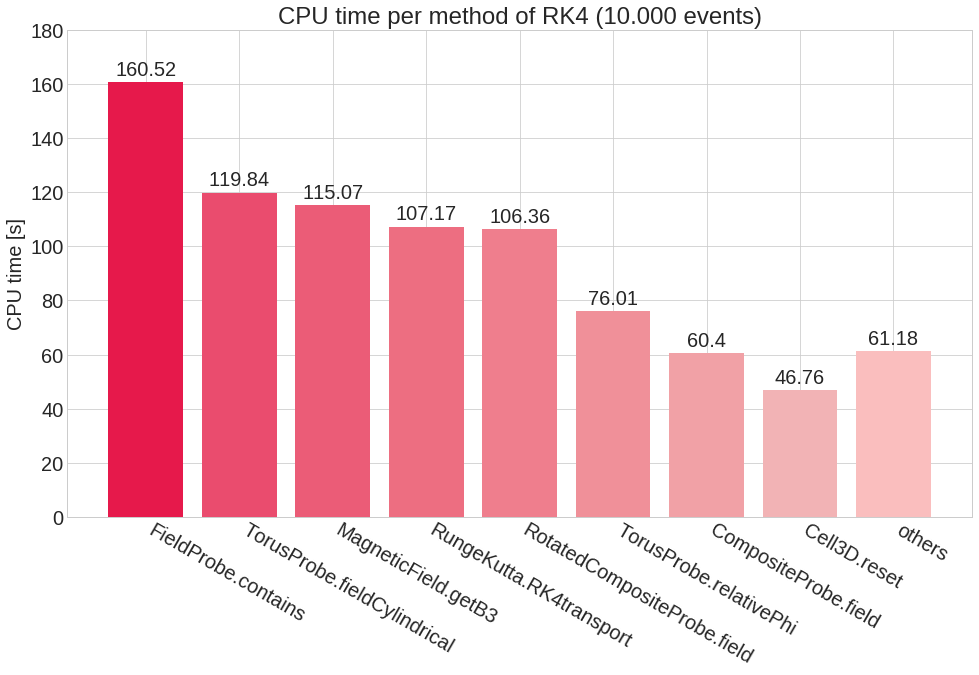
\includegraphics[scale=0.44]{bfield/rk4_composition}
        \caption{\label{fig:rk4_composition} CPU times consumed by each Runge Kutta 4 component.}
    \end{figure}

As seen in Figure \ref{fig:rk4_composition}, most of the Runge Kutta 4 algorithm's runtime is actually used by methods retrieving the magnetic field from the \texttt{swimmer} package.
These methods' purposes is to compute the magnetic field $\textbf{B}(x,y,z) = \langle \operatorname{B_1}(x,y,z),\operatorname{B_2}(x,y,z),\operatorname{B_3}(x,y,z)\rangle$ at a specific $(x,y,z)$ point inside the CLAS12 detector, which is done by placing virtual ``probes'' inside it. % Note: Maybe I should elaborate more on this.

To accelerate this computation, the possibility of using trilinear interpolation~\cite{bourke1999interpolation} for $\mathbf{B}$ was analyzed.
The option was considered favorable since the imprecision brought by interpolating the value instead of directly computing it could be diminished by the \textbf{update} part of the KF and by only using the interpolated magnetic field in a fixed number of iterations of the KF before using the real magnetic field for the remaining ones.
Appendix \ref{add:trilinear_interpolation} describes how trilinear interpolation works.

The algorithm used is a direct transcription of the definition of trilinear interpolation, and is defined in two steps.
First, obtain the regular grid and the measurements at each border, which is done by selecting a grid size $\left([\text{min}_x, \text{max}_x], [\text{min}_y, \text{max}_y], [\text{min}_z, \text{max}_z]\right)$ from which the magnetic field measurements are taken with step sizes defined as $\{\text{ss}_x, \text{ss}_y, \text{ss}_z\}$.
These parameters define a regular tridimensional grid and a measurement for the magnetic field for each point in this grid is obtained.

For the second step, the specific measurement in the location desired is obtained by evaluating the formula defined in \ref{add:trilinear_interpolation}.
In the case that the location is outside the range of the regular grid, the real magnetic field is computed for that point.

After the interpolation algorithm was implemented, the borders and the step size of the grid were left as parameters to be tuned.
First, $[\text{min}_z, \text{max}_z]$ were set to $[229 \text{cm}, 569 \text{cm}]$ since these are the limits of the $z$ variable in the detector.

    \begin{figure}[ht]
        \centering
        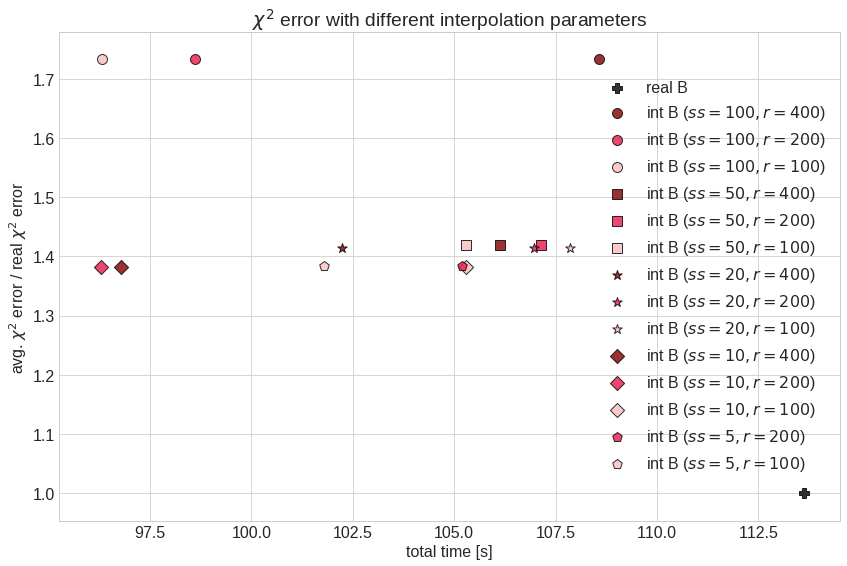
\includegraphics[scale=0.52]{bfield/chi2_vs_time}
        \caption{\label{fig:bfield_chi2_vs_time} $\chi^2$ error when doing the track fitting with the interpolated magnetic field divided by the obtained when using the real magnetic field vs required time. ``real B'' is the real magnetic field while ``int B'' is the interpolated magnetic field with its parameters in parentheses.}
    \end{figure}

To set the step size for each variable, $\text{ss}$ is defined such that $\text{ss} = \text{ss}_x = \text{ss}_y = \text{ss}_z$ for simplicity.
Then, the range $[\text{min}, \text{max}]$ and the variable $r$ are defined such that $\text{min} = \text{min}_x = \text{min}_y$ and $\text{max} = \text{max}_x = \text{max}_y$ and $r = \text{max} = \text{-min}$, to take advantage of the symmetries of the detector, which can be seen in Figures \ref{fig:dc_horizontal_cut} and \ref{fig:dc_vertical_cut} from Section \ref{ssec:framework_dc}.

Tests are ran by running the software using the interpolated magnetic field with different combinations of parameters, comparing them using the division of the $\chi^2$ error obtained by the one found when running the real field and measuring it against the time it takes to run the program.
The results are averaged over a set of $2.500$ estimated tracks and the results can be seen in Figure \ref{fig:bfield_chi2_vs_time}.
It is worth noting that some outliers are removed from the figure to aid with visualization.
The tested values for each were the following:
    \begin{align*}
        \text{ss} &\in \{5 \text{cm}, 10 \text{cm}, 20 \text{cm}, 50 \text{cm}, 100 \text{cm}, 200 \text{cm}\}\\
        r &\in \{100 \text{cm}, 200 \text{cm}, 400 \text{cm}\}
    \end{align*}

As seen in the figure, the interpolation parameters that provide the best results are $\text{ss} = 10 \text{cm}$ and $r = 200 \text{cm}$.

    \begin{figure}[ht]
        \begin{floatrow}
            \ffigbox[0.48\textwidth]{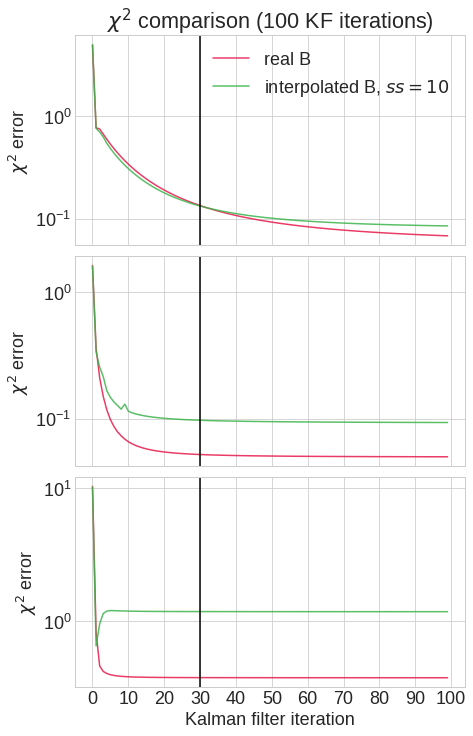
\includegraphics[height=0.72\textwidth] 
            {bfield/chi2_real_vs_ss10}}
                {\caption{\label{fig:bfield_real_vs_ss10} $\chi^2$ error comparison between real magnetic field and interpolated one with a step size of $10$ running the KF with $100$ iterations. A vertical black line denotes the $30$ usual KF iterations.}}
                
            \ffigbox[0.48\textwidth]{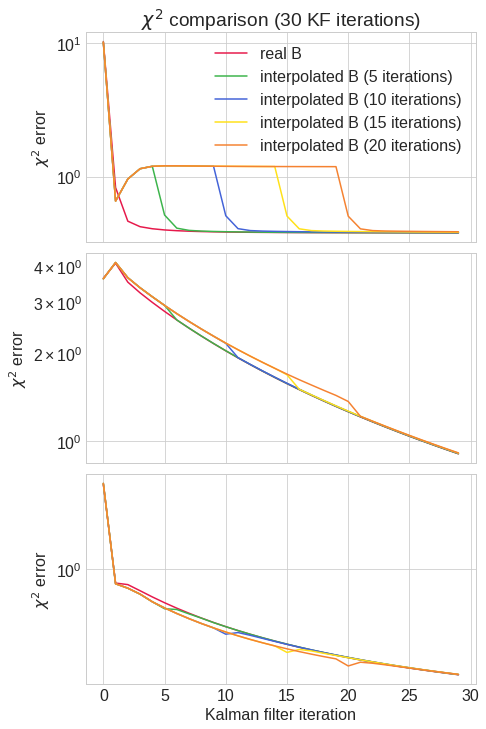
\includegraphics[height=0.72\textwidth] {bfield/chi2_real_vs_ni20}}
                {\caption{\label{fig:bfield_real_vs_ni20} $\chi^2$ error comparison between the real magnetic field and the interpolated one for different numbers of iterations running the KF with $30$ iterations.}}
        \end{floatrow}
    \end{figure}

Figure \ref{fig:bfield_real_vs_ss10} then shows the $\chi^2$ error of three distinct tracks running $100$ KF iterations, contrasting the error of the real magnetic field to that of the selected interpolated version.
As can be seen the figure, in most cases both version converge similarly but the one using the real magnetic field provides better results, albeit generally taking up more time.

Finally, a compromise that still provides good results is reached by running only the first KF iterations using the interpolated magnetic field and the last ones using the real one.
The number of iterations using the interpolated field tested are $0$, $5$, $10$, $15$, $20$, $25$ and $30$, but at the end all but the last one end up with the same final $\chi^2$ error.
Due to this, the number of interpolated magnetic field steps is decided based on the total DCHB and DCTB times when using each version, as presented in Table \ref{tab:interpolated_steps_times}.

It is worth noting that the total times per event listed here are slightly different than the ones presented in the validations of the method, and this is because these tests were ran on $3.000$ events instead of the usual $10.000$.
This decision is taken for the sake of expediency and because it shouldn't affect the results in a significant manner.

    \begin{table}[ht]
        \centering
        \begin{tabular}{@{}l|ll@{}}
        \toprule
        Name                  & DCHB time [s] & DCTB time [s] \\ \midrule
        Real magnetic field   & 130.42        & 48.78         \\
        5 interpolated steps  & 133.42        & 52.05         \\
        10 interpolated steps & 110.94        & 42.24         \\
        15 interpolated steps & 107.87        & 40.76         \\
        20 interpolated steps & 103.83        & 38.46         \\
        25 interpolated steps & 109.52        & 40.14         \\
        30 interpolated steps &  96.63        & 35.14         \\ \bottomrule
        \end{tabular}
        \caption{\label{tab:interpolated_steps_times} DCHB and DCTB times [s] using different interpolated steps.}
    \end{table}

As can be seen in Table \ref{tab:interpolated_steps_times}, the best times were obtained by running $30$ interpolated steps, but the final number of interpolated steps set in the code are $20$, the second best.
This decision is taken due to the fact that, as can be seen in Figure \ref{fig:bfield_real_vs_ni20}, if no steps are taken with the real magnetic field, the final $\chi^2$ error is much higher than the original one.
Figure \ref{fig:bfield_real_vs_ni20} shows the $\chi^2$ error obtained by using this method.

It's worth noting that the interpolation is only implemented in the Hit-Based tracking part of the KF since the Time-Based part requires as much precision as possible.
% Note: This could use a citation but it came from a meeting with Veronique. It's due to the fact that DCTB analyzes using a much finer grain than DCHB, and DCHB is mostly used to quickly filter tracks so that DCTB doesn't need to analyze all of them.
% \newpage
\subsection{Multithreaded Cluster and Track Finding Algorithms} \label{ssec:prop_multithreaded_ctf}
A multithreaded algorithm is an algorithm that takes advantage of the fact that most modern CPUs have more than one core, thus allowing them to concurrently run various execution threads on these multiple cores in order to take less time processing the same data. % Note: Maybe I should cite a book on this.
This is especially useful in the context that the CLAS12 software is ran at JLab, where many data events are computed concurrently, in different machines.
To understand why a multithreaded approach is useful, a bit of insight is needed on how the work in the CLAS12 execution hardware is distributed:

First, a number of threads per engine $T$ is defined in the CLARA configuration file, allowing for $T$ instances of the same engine to process different data events in the different cores at the same time.
Then, if the number of engines running in the production chain is $E$, at most a number of $T\cdot E$ threads will be running at the same time in the HPC cluster.
Dubbing the number of cores at the cluster $C$, a well-tuned configuration file is set so that $T\cdot E \approx C$ so as to utilize the cluster's capacity as best as possible.

Ideally, this setup would work in such a way that all the $C$ cores remain constantly running, but a problem arises due to the fact that the CLAS12 engines require to run in a sequential manner and, as seen in Figure \ref{fig:engines-times-sep2018} from Section \ref{ssec:prob_the_problem}, each engine takes a vastly different amount of time to run.
Because of this, the cores running the faster engines will be left waiting for the slower ones that come previous to them to finish their execution.

Based on this reasoning, a valid approach for accelerating the software is to distribute the work done in the slowest engines, DCHB and DCTB, onto more threads so that the computing time is improved and a better use of the available hardware is ensured.
Two methods for taking advantage of this idea are proposed: A multithreaded algorithm to use in cluster finding and one to use in track finding.

\textbf{Multithreaded Cluster Finding Algorithm}: Analyzing the cluster finding algorithm described in Section \ref{ssec:framework_cf}, it can be seen that there is no reason to do the \textbf{Clump Finding} step before the \textbf{Hit Prunning} one, considering that the second iterates through the hits on a layer-by-layer basis instead of based on the clumps found by the first.

Then, the \textbf{Out-of-Timers Removal}, the \textbf{Cluster Fitting} and the \textbf{Cluster Splitting} steps can be ran in parallel by assigning a thread to each clump found.
It is in theory possible to further parallelize the algorithm by assigning individual threads to each cluster found in the Cluster Splitting step and running the fitting done to them separately, but the estimated gain in computing time is very small due to the fact that only one fit is done on the split clusters, so the option was discarded.

\textbf{Multithreaded Track Finding Algorithm}: The track finding done in the DC code described in Section \ref{ssec:framework_tf} requires a set of measurements to run, which are taken from the hits in six different clusters.
Due to the geometry of the DC detector (which can be seen in Figure \ref{fig:dc_horizontal_cut} from Section \ref{ssec:prob_context}), finding pairs of clusters (dubbed crosses) in the two superlayers that conform a sector is trivial.

Then, all the combinations of three crosses that could potentially make sense as being formed by a particle's trajectory are considered different, independent tracks.
Via the Kalman filter, a fit is attempted for each of these tracks to find the ones that are most likely to be formed by an actual particle passing through the detector.
Considering that each track is fit separately and that they are independent from each other, a multithreaded algorithm is implemented where all the tracks in a data event are fit concurrently in different threads.
% \newpage
% \subsection{Fourth Order Adams-Bashforth-Moulton Method Proof of Concept} \label{ssec:prop_abm}
% Explain why it's a good idea, the separation between two regions and the amount of measurements with a regular step size that can be taken.
As can be seen in figure \ref{fig:dc_horizontal_cut} from subsection \ref{ssec:framework_dc}, the measurements can be divided in the three regions due to the geometry of the detector.
While most of the distances between measurements are usually at most $4$ or $5$ [cm], the distance between regions can be more than a meter.
Also, due to the way that the Kalman Filter works, after transporting the state vector from the first measurement site to the last, this vector needs to be transported back to run the KF again, which requires it to be moved for around $3.5$ meters.

Currently, this movement of the state vector is done through Runge Kutta 4, as is described in subsection \ref{ssec:framework_dc} with a step size $h=1$ so that the $z$ variable is updated by one centimeter in each RK4's iteration, occasionally updating it by $2$ [cm] when the magnetic field at that point is small enough.
Considering that for most particles the majority of the movement from regions $1$ to $2$, $2$ to $3$ and from $3$ back to $1$ the step size is kept at $1$ [cm], the option of changing RK4 for the Fourth order Adams-Bashforth-Moulton (ABM4) method is evaluated.

% Quickly explain the method itself and reference the addendum where it's explained in more detail.
ABM4 is a multi-step method used to solve initial value problems described in detail in \ref{add:abm4}.
The method can solve the same kind of problems as RK4, but it has the advantage that it only requires to evaluate the $\mathbf{f}(z,\mathbf{x})$ function once per iteration, whereas RK4 does this four times.

% Explain a little bit the implementation itself, how RK4 must be used 3 times at the beginning and one time by the end.
The change does not come without disadvantage however, since it requires the use of four previous steps to compute the next one as can be seen in equations \eqref{eq:abm4_explicit} and \eqref{eq:abm4_implicit} from the referenced addendum.
Due to this the step size must be kept constant through each step.
A common and simple-to-execute solution for this is to run RK4 for three steps after the initial state vector, and thus this option is implemented.
It's worth noting that due to the particular conditions of the problem, $z_{k+1}$ does not necessarily fulfill the condition that $z{k+1} = z_k + n h$ where $n$ is an arbitrary natural number, so it's usually impossible to reach the next measurement site from the last one using ABM4, but this is easily fixable by using RK4 at the last step of the process.

% TODO: TALK WITH CT AND SEE IF HE AGREES THAT WE SHOULD SCRAP THIS FOR THE TIME BEING AND MAYBE EXPLORE THE OPTION IN THE FUTURE.

% Explain why the algorithm couldn't be implemented; mention the error associated to the lack of magnetic field differentials.
% After the initial analysis is done, ABM4 is integrated into the code instead of RK4 and tests are ran, but the results are not as good as are expected, as can be seen in figure \textbf{TODO}. % TODO: Add a figure showing the huge errors in the state vector.
% This error is attributed to the issue with the implementation of the equations of motion that is expressed in subsection \ref{ssec:framework_tf}, where equations \eqref{eq:tf_dtx_dx}, \eqref{eq:tf_dtx_dy}, \eqref{eq:tf_dty_dx} and \eqref{eq:tf_dty_dy} cannot be implemented correctly because of the fact that the differentials of the magnetic field $\textbf{B}(x,y,z)$ are unknown, which introduces an instability to the method which causes it to converge to different results when compared to RK4. % TODO: If I'm gonna say that the method didn't work I'm gonna need a better explanation into why I think this is true.

% Still, considering that the theory checks up ABM4 can potentially work in contexts such as this for other particle detectors, and it can be a good idea to try and implement the method if additional information about the system is known in the future.
\newpage
\subsection{Multithreaded Kalman Filter Algorithm Proof of Concept} \label{ssec:prop_multithreaded_kf}

    \begin{wrapfigure}{r}{0.51\textwidth}
        \centering
        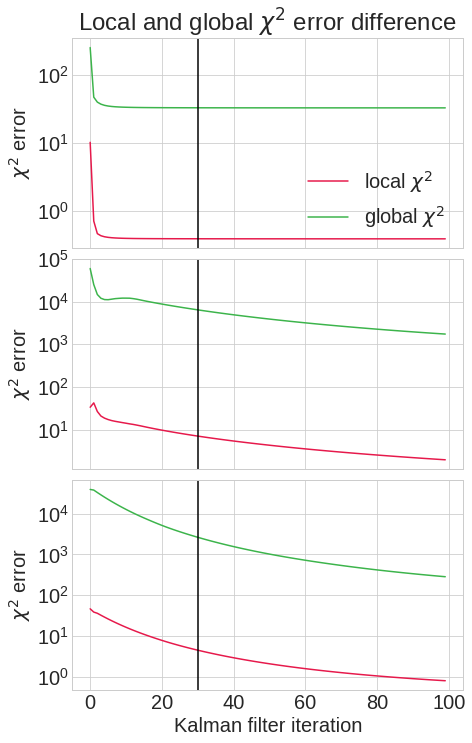
\includegraphics[width=1\textwidth]{multithreaded_kf/chi2error}
        \caption{\label{fig:mkf_chi2error} Local and global $\chi^2$ errors for a track in events \#$5$, \#$67$ and \#$103$ for $100$ KF iterations. The $30$ KF iterations commonly computed are marked by a black vertical line.}
    \end{wrapfigure}

A multithreaded Extended Kalman Filter (EKF) variant is proposed to accelerate the computation of the EKF in the code and to potentially obtain better solutions.
To understand why this option is deemed useful, it has to be noted that the EKF implementation described in Section \ref{ssec:framework_tf} contains a hardcoded stopping point for the EKF after $30$ iterations, with no dynamic analysis onto how good the solution found up to that point is or if the methods used have already converged.
Changing this might open the possibility of a multithreaded algorithm.

% DYNAMIC STOPPING POINT
Due to this, the first efforts were placed on finding this dynamic stopping point for the algorithm.
Naturally, this criteria must be related to the $\chi^2$ error, which is the variable that is being minimized by the method.
As mentioned before, a deifnition of the $\chi^2$ error is given in Appendix \ref{add:errors}.

The problem with this approach is that for every iteration of the EKF only the so-called ``local'' $\chi^2$ error is computed, while the ``global'' one is only computed once the EKF has finished.

% Note: if it's too hard to understand the local and global $\chi^2$ error then it might be better to leave this out for good.
The local $\chi^2$ error is computed while the EKF is running by projecting the state vector at a measurement site into the measurement itself and computing the squared difference divided by the uncertainty of the measurement.
The problem with this version of the error is that as the EKF runs, each state vector changes, and thus the error computed is different from the real one.

The global $\chi^2$ error is this ``real'' one, where each state vector near a measurement site is projected into it and the error is calculated.
The reason that the global error is only computed after the EKF has ran is that the process of updating the state vector across the particle trajectory is computationally-intensive, and thus doing it for each iteration of the EKF would be too expensive for the total computing time.

The problem that arises from this concept is that there are tracks where the convergence of the local $\chi^2$ error is not representative of the converge of the global one.
As can be seen in the first EKF iterations in the track from event \#$67$ in figure \ref{fig:mkf_chi2error}, the local and the global $\chi^2$ errors are not always correlated. % Note: I should find events where this lack of correlation is more apparent.

    \begin{figure}[ht]
        \centering
        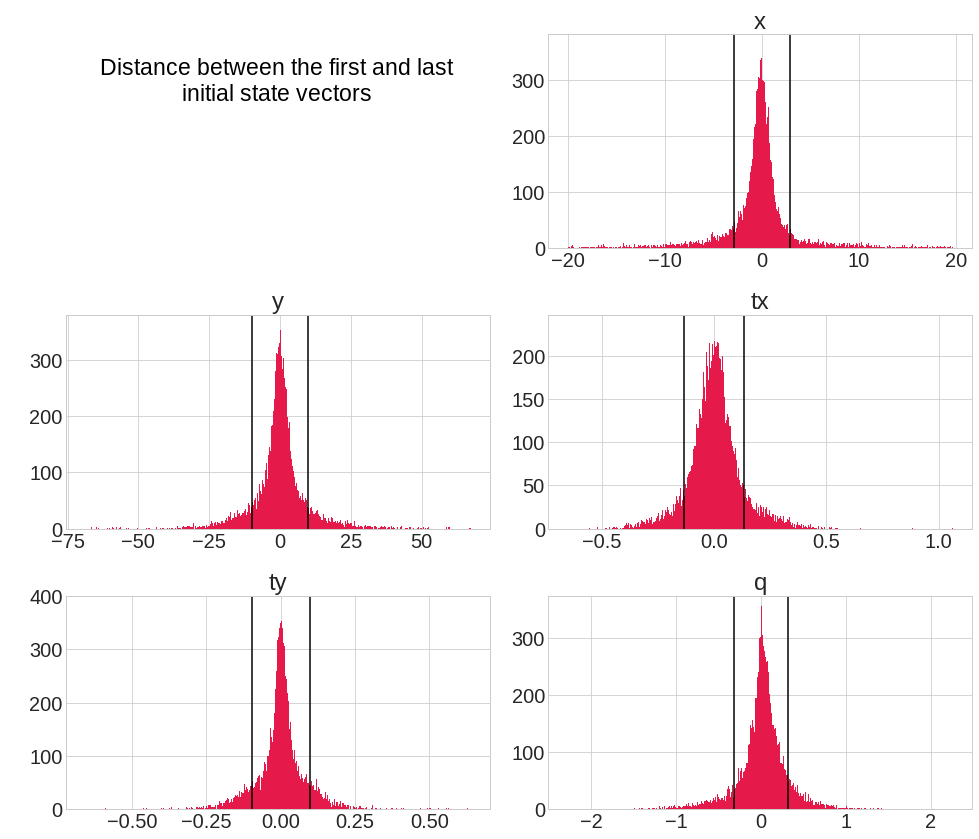
\includegraphics[scale=0.44]{multithreaded_kf/isv_distance}
        \caption{\label{fig:mkf_isv_distance} Distance between the first and the last initial vectors for the tracks found in $10.000$ events. The black lines mark a region where $80\%$ of the distances are contained.}
    \end{figure}

Then, the idea of computing different initial state vectors $\mathbf{x}(z) = \left<x, y, \theta_x, \theta_y, q\right>$ in parallel for each track was considered.
These different initial state vectors should be consistent, and this is pursued by comparing the different variables from the first and the last state vectors used by the Kalman filter.
This difference is recorded for all the tracks found in $10.000$ events and its distribution is evaluated.
A plot of this distribution for each variable in the state vector can be seen in Figure \ref{fig:mkf_isv_distance}.

    \begin{wrapfigure}{r}{0.51\textwidth}
        \centering
        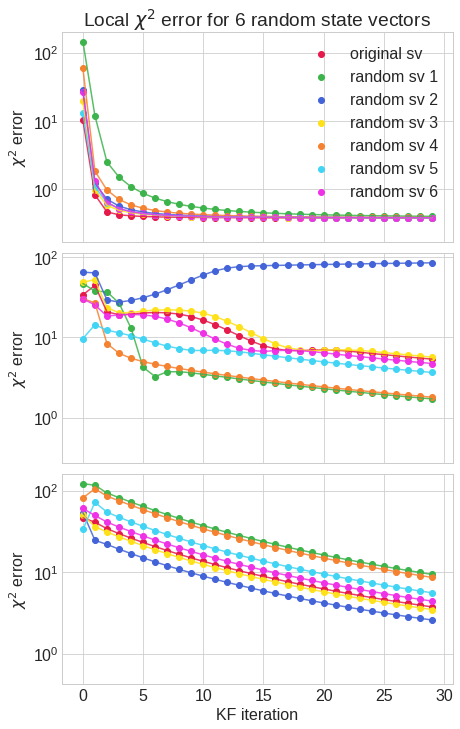
\includegraphics[width=1\textwidth]{multithreaded_kf/mkf_test}
        \caption{\label{fig:mkf_test} Local $\chi^2$ errors starting from $6$ random initial state vectors compared with the original in events \#$5$, \#$67$ and \#$103$ for $30$ KF iterations.}
    \end{wrapfigure}

To generate the initial state vector for the KF to run, a random perturbation inside a range that captures $80\%$ of the distance values (denoted as black vertical lines in Figure \ref{fig:mkf_isv_distance}) is added to the initial state vector and multiple instances of the KF are ran with these different initial state vectors. The resulting $\chi^2$ error obtained by running the KF in this manner for $6$ random initial state vectors can be seen in Figure \ref{fig:mkf_test}.

As can be seen in the figure, for the tracks in events $67$ and $103$ the final $\chi^2$ obtained from a random initial state vector was better than the one obtained for the original.
Special attention should be given to the ones obtained by the random state vectors $1$ and $4$ from event $67$ which are close to a fifth of the original one found.

% INCREASED POWER CONSUMPTION
It's worth noting that if a dynamic stopping point is implemented, that is to say, a point in which the KF is stopped before reaching the $30$ iterations, the multithreaded algorithm may provide better results in the same amount of time as the original one.

It's worth noting that while this algorithm may be able to provide better results in the same amount of time, the approach actually increases the total CPU-time and power consumption required to run the software.
This is due to the fact that multiple instances of the KF run in parallel.
In the case of the CLAS12 software as is ran in JLab, this additional power consumption meant that the algorithm was programmed but not implemented in the code due to power constraints.